\documentclass[11pt, a4paper]{scrartcl}

\usepackage{listings}
\usepackage{jlcode}
\usepackage{color}
\usepackage[utf8]{inputenc}
\usepackage{hyperref}
\usepackage{graphicx}

\title{Julia Installationsanleitung für Linux}
\author{}
\date{}

\definecolor{dkgreen}{rgb}{0,0.6,0}
\definecolor{dkblue}{rgb}{0,0,0.4}
\definecolor{gray}{rgb}{0.5,0.5,0.5}
\definecolor{mauve}{rgb}{0.58,0,0.82}

\hypersetup{
    colorlinks=true,
    linkcolor=black,
    urlcolor=dkblue,
}
\lstset{
	language=Julia,
%	frame=tb,
	aboveskip=3mm,
	belowskip=3mm,
	showstringspaces=false,
	columns=flexible,
	basicstyle={\small\ttfamily},
	numbers=none,
	numberstyle=\tiny\color{gray},
	keywordstyle=\color{blue},
	commentstyle=\color{dkgreen},
	stringstyle=\color{mauve},
	breaklines=true,
	breakatwhitespace=true,
	tabsize=3
}



\begin{document}
	\maketitle
	
	
	
	
	
	
	\section{Julia als Binaries herunterladen und installieren}
%	\href{http://julialang.org}{julialang.org}
%	\url{http://julialang.org}
	Öffnen Sie die Webseite \url{https://julialang.org/downloads/} in ihrem Browser. Klicken Sie dort auf den entsprechenden Link mit der Bezeichnung \texttt{64-bit} bei \texttt{Generic Linux Binaries}, um die Julia Binaries herunterzuladen.
	
	\begin{figure}[h!]
		\centering
		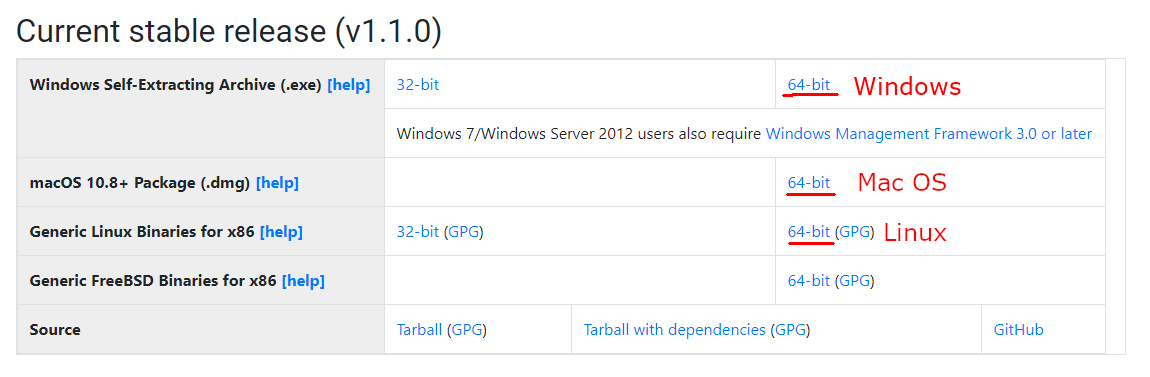
\includegraphics[width=\textwidth]{imgs/download.png}
	\end{figure}

	Extrahieren Sie den enthaltenen \texttt{julia-1.1.0} Ordner in einen Pfad Ihrer Wahl -- damit ist Julia jetzt bei Ihnen installiert.
	
	
	
	
	
	
	
	
	
	
	
	
	
	
	\newpage
	\section{Das erste Mal Julia}
	Starten Sie Julia aus Ihrem Terminal heraus indem Sie die Datei \texttt{bin/julia} in dem (im vorherigen Schritt) extrahierten Ordner ausführen. Ihr Terminal sollte jetzt so ähnlich aussehen (Dateipfade können abweichen):
	
	\begin{figure}[h!]
	\centering
	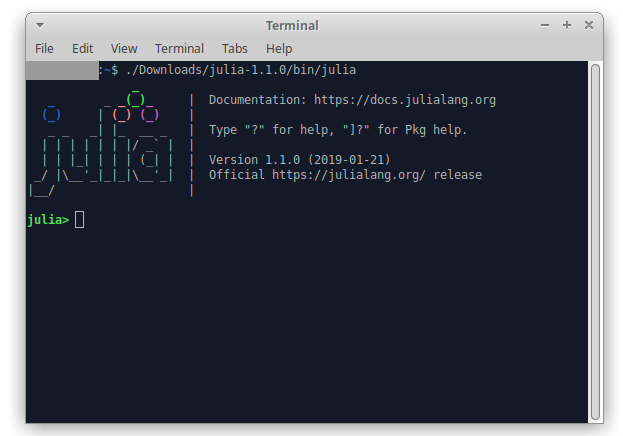
\includegraphics[width=0.7\textwidth]{imgs/julia_REPL.png}
	\end{figure}

	Dies ist die Julia Konsole (auch Julia REPL genannt). Sie ist eine Möglichkeit Julia zu verwenden. Geben Sie zum Test
	
	\begin{lstlisting}
		3+3
	\end{lstlisting}
	
	ein und führen Sie den Befehl per \texttt{Enter}-Taste aus. Sie sollten nicht überraschend das Ergebnis 6 erhalten.
	
	\vspace{1cm}
	
	Auch wenn die Konsole prinzipiell genügt um in Julia zu Programmieren, ist sie doch sehr rudimentär. Im folgenden wollen wir eine viel schickere und Benutzerfreundlichere Julia Oberfläche installieren.
	
	
	
	
	
	
	
	
	
	
	
	\newpage
	\section{IJulia installieren}
	
	Zusätzlich zur Programmiersprache Julia wollen wir noch IJulia und Jupyter installieren, um Julia bequem im Browser in sogenannten Notebooks verwenden zu können. Grob gesagt ist Jupyter eine Notebook Oberfläche für verschiedene Programmiersprachen und IJulia die Schnittstelle zwischen Julia und Jupyter. 
	
	
	Zunächst werden wir in dieser Sektion IJulia installieren. Führen Sie folgenden Befehl in der Julia Konsole aus, indem Sie ihn abtippen (Kopieren und Einfügen ist in der Julia Konsole nicht ganz einfach) und mit der \texttt{Enter}-Taste bestätigen.
	
	\begin{lstlisting}
		using Pkg; Pkg.add("IJulia");
	\end{lstlisting}

	Sie sollten folgende Ausgabe erhalten (die Dateipfade können abweichen):
	
	\begin{figure}[h!]
	\centering
	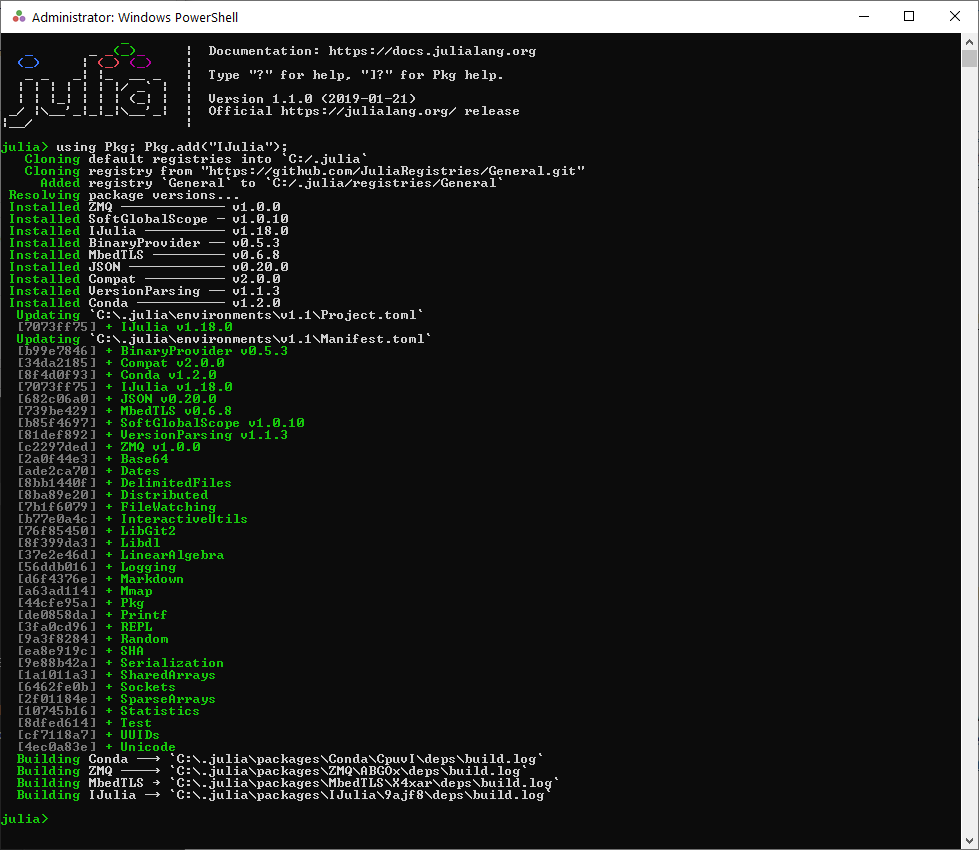
\includegraphics[width=0.9\textwidth]{imgs/IJulia_install.png}
	\end{figure}

	IJulia ist nun erfolgreich installiert.
	
	
	
	
	
	
	
	
	
	
	
	
	
	\section{Jupyter installieren und das erste Mal starten}
	
	Um Notebooks erstellen oder öffnen zu können, muss grundsätzlich zuerst immer Julia geöffnet, IJulia geladen und dann der Jupyter Notebook Server gestartet werden. Im Folgenden wird der erstmalige Vorgang beschrieben, der auch die automatische Installation von Jupyter beinhaltet. 
	
	Stellen Sie sicher, dass Sie eine Julia Konsole geöffnet haben und führen Sie darin folgenden Befehl aus:
	
	\begin{lstlisting}
	ENV["JUPYTER"]=""; ENV["PYTHON"]=""
	using IJulia; notebook()
	\end{lstlisting}
	
	Die erste Zeile wird nur vor der ersten Installation benötigt. Hier wird Julia selbst mittels \texttt{ENV["JUPYTER"]=""} und \texttt{ENV["PYTHON"]=""} mitgeteilt, dass es keine bestehende Jupyter oder Python Versionen suchen sondern selbst eine neue Version installieren soll, sofern benötigt.
	
	Der nachfolgenden Befehl, \texttt{using IJulia}, lädt IJulia und versucht den Jupyter Notebook Server mittels \texttt{notebook()} zu starten. Julia wird feststellen, dass dieser beim ersten Start noch nicht installiert ist, und fragt uns, ob es Jupyter für uns installieren soll:
	
	\begin{figure}[h!]
	\centering
	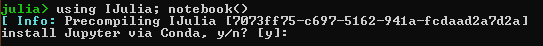
\includegraphics[width=0.9\textwidth]{imgs/Jupyter_install.png}
	\end{figure}
	
	Dies bestätigen wir mit einem Druck der \texttt{Enter}-Taste. Die Installation von Jupyter kann einige Minuten in Anspruch nehmen.
	
	Nach Abschluss der Installation sollte sich automatisch der Browser öffnen und das Jupyter Notebook Interface erscheinen (Ordner, Dateien und Sprache können abweichen):
	
	\begin{figure}[h!]
	\centering
	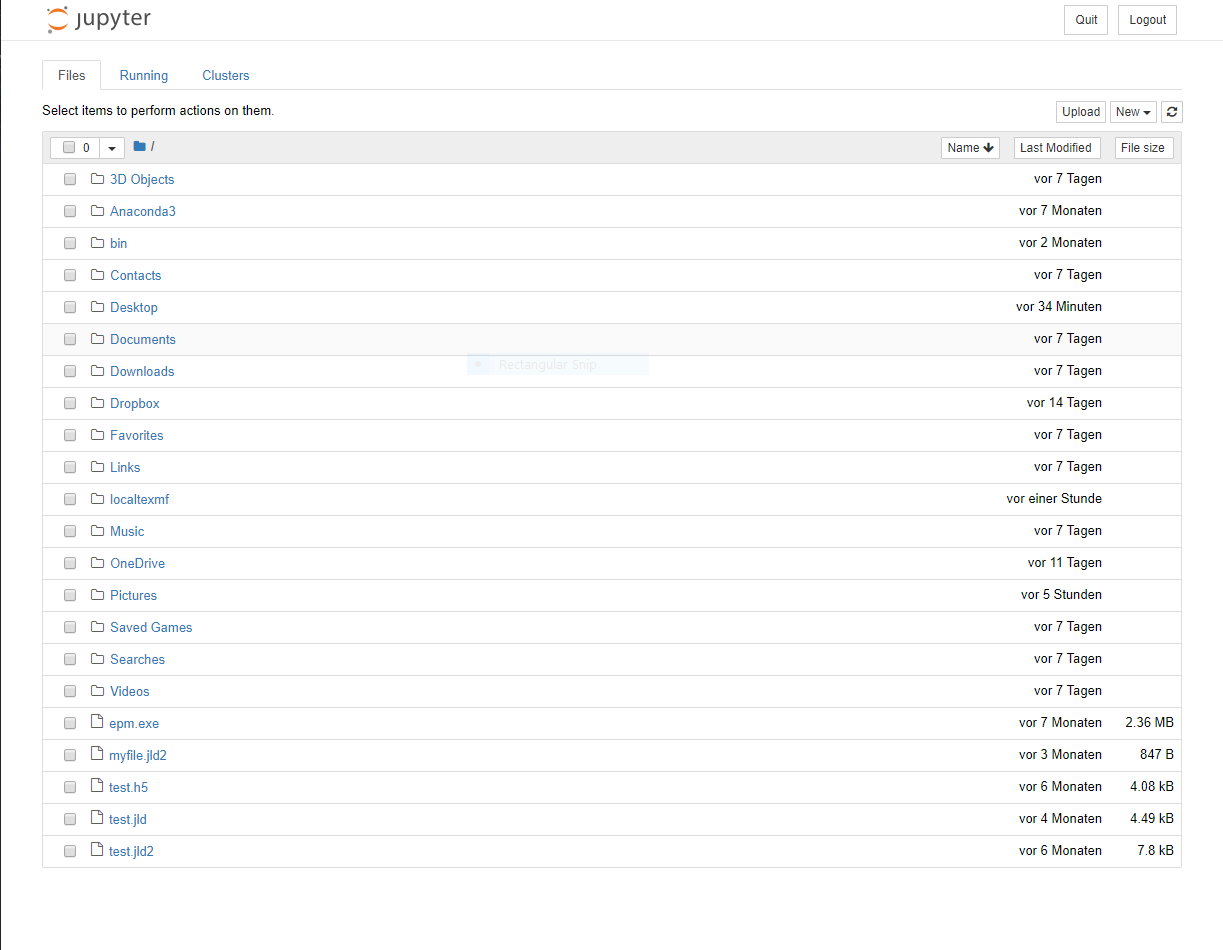
\includegraphics[width=0.5\textwidth]{imgs/jupyter.png}
	\caption{Die Startseite des Jupyter Interfaces. \label{fig:jupyter}}
	\end{figure}
	
	Der Server läuft solange die Julia Konsole im Hintergrund geöffnet ist. Sobald wir diese schließen, wird der Server gestoppt.
	
	
	
	
	
	
	
	
	
	
	
	
	
	\newpage
	\section{Einfacher Test der Notebook Oberfläche}
	
	Klicken Sie in der Jupyter Oberfläche (Fig. \ref{fig:jupyter}) rechts oben auf den Button \texttt{New} und klicken Sie danach im sich öffnenden Kontextmenü auf den Eintrag \texttt{Julia 1.1.0}. Es sollte sich nun ein frisches Jupyter Notebook öffnen:
	
	\begin{figure}[h!]
	\centering
	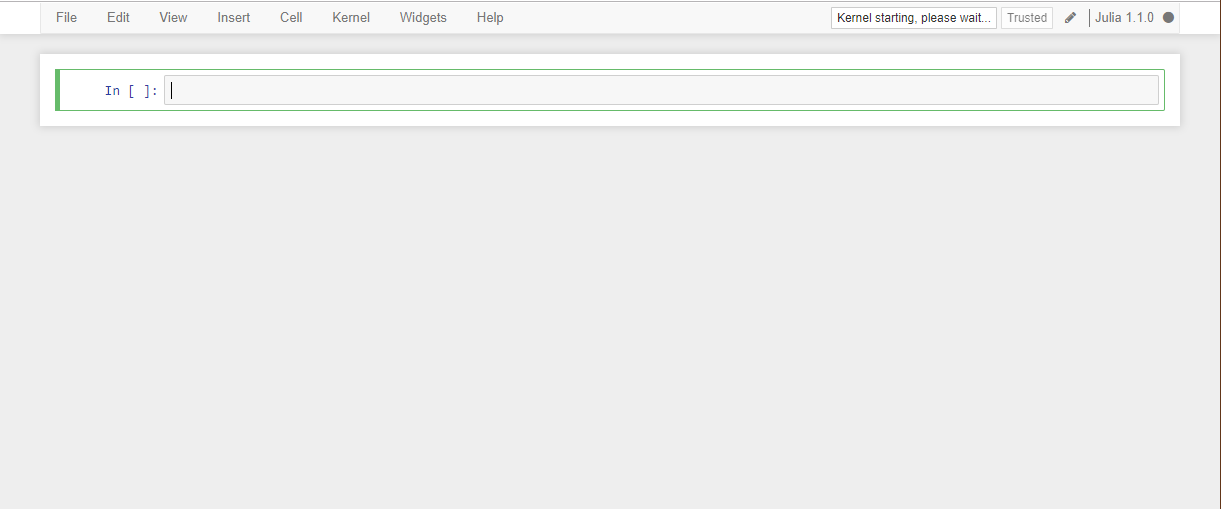
\includegraphics[width=0.9\textwidth]{imgs/jupyter_notebook.png}
	\end{figure}

	Klicken Sie in die erste (und einzige) Zelle des Notebooks und geben Sie dort
	
	\begin{lstlisting}
	3+3
	\end{lstlisting}
	ein. Führen Sie die Zelle per \texttt{SHIFT + ENTER} aus (gleichzeitiges Drücken der \texttt{SHIFT} bzw. \texttt{UMSCHALT} und der \texttt{ENTER} Taste). Es sollte das Ergebnis \texttt{6} erscheinen:

	\begin{figure}[h!]
	\centering
	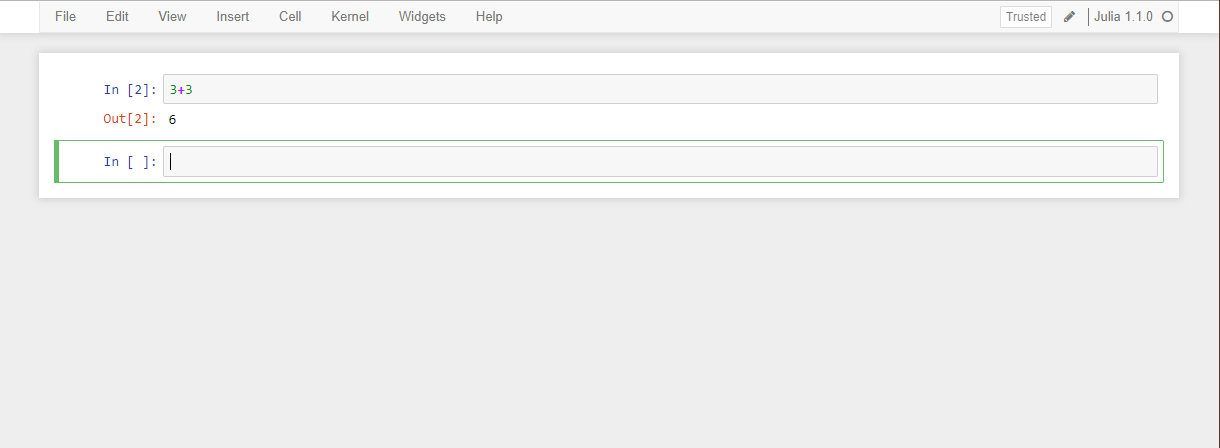
\includegraphics[width=0.9\textwidth]{imgs/jupyter_notebook_test.png}
	\end{figure}	

	Die Installation von Julia, IJulia und Jupyter war also erfolgreich und die Computer-Physik kann beginnen!
	
	

	\newpage
	\section{Optional: Julia zum \texttt{PATH} hinzufügen / Julia global in der Konsole verfügbar machen}
	
	Damit Julia global in der Konsole per \texttt{julia} gestartet werden kann, muss es in Ihrer Umgebungsvariable \texttt{PATH} vorkommen. Sie haben dafür mehrere Möglichkeiten.
	
	
	\subsection{Symbolischer Link}
	
	Fügen Sie in \texttt{/usr/bin} einen symbolischen Link hinzu, der zu der Datei \texttt{bin/julia} in dem von Ihnen extrahierten Ordner führt. Dies können Sie mittels
		
	\begin{lstlisting}[language=bash, columns=fixed, breaklines=false]
	ln -s PATH_TO_JULIA_BINARIES/bin/julia /usr/bin/julia
	\end{lstlisting}
	
	in Ihren Terminal durchführen.
	
	 
	 
	\subsection{Verändern der \texttt{.bash\_profile} Datei}
	
	Fügen Sie dafür die folgende Zeile am Ende der Datei \texttt{.bash\_profile} in Ihrem Home-Verzeichnis ein:
	
	\begin{lstlisting}[language=bash, columns=fixed, breaklines=false]
	export PATH="PATH_TO_JULIA_BINARIES/bin:$PATH"
	\end{lstlisting}
	
	Sie können dafür einen beliebigen Texteditor verwenden.
	
	Konkret können Sie beispielsweise so vorgehen:
	
	\begin{itemize}
		\item Öffnen Sie ein Terminal.
		\item Führen Sie den Befehl 
		\begin{lstlisting}[language=bash, columns=fixed, breaklines=false]
		vim .bash_profile
		\end{lstlisting}
		aus. Es öffnet sich der Konsolen-Text-Editor vim. (Eventuell ist die angezeigte Datei leer. Die nachfolgenden Schritte sollten aber in jedem Fall funktionieren)
		\item Drücken Sie \texttt{SHIFT + G} (\texttt{UMSCHALT + G}), lassen Sie die Tasten los, und drücken Sie dann direkt die Taste \texttt{o} (der Buchstabe nicht die Zahl). (Sie sollten so ans Ende der Datei gesprungen sein und dort eine neue Zeile eingefügt haben.)
		\item Fügen Sie nun die oben genannte Zeile ein (am besten abtippen!).
		\item Drücken Sie die \texttt{ESC} Taste. Tippen Sie dann \texttt{:wq} ein und bestätigen Sie mit \texttt{ENTER}. (Ihre Eingabe sollte am unteren Rand erscheinen.)
	\end{itemize}
	
	Wenn Sie nun das Terminal schließen und neu öffnen sollte julia per Befehl \texttt{julia} gestartet werden können.
	
	
\end{document}